\documentclass[11pt,a4paper]{article}
\usepackage[margin=25mm]{geometry}
\usepackage{graphicx,booktabs,amsmath,hyperref,fancyhdr}
\hypersetup{hidelinks,pdftitle={Bangla Sign Language Gesture Recognition},pdfauthor={Nazmul Hassan}}
\pagestyle{fancy}\fancyhf{}\fancyhead[L]{\small Bangla Sign Language Gesture Recognition}\fancyfoot[C]{\thepage}
\setlength{\emergencystretch}{2em}\setlength{\headheight}{14pt}\setlength{\parskip}{4pt}\setlength{\parindent}{0pt}
\title{Bangla Sign Language Gesture Recognition:\\Static Image Classification and Bounded Sentence Recognition}
\author{Nazmul Hassan\\Department of Electrical and Computer Engineering\\North South University, Dhaka, Bangladesh\\\small ROR: \href{https://ror.org/05wdbfp45}{05wdbfp45}\\\small ORCID: 0000-0001-6116-017X\\\small \href{mailto:iam.najib@yahoo.com}{iam.najib@yahoo.com}}
\date{\small Preprint}

\renewcommand{\topfraction}{.9}\renewcommand{\textfraction}{.05}\renewcommand{\floatpagefraction}{.85}
\makeatletter
\renewcommand{\@seccntformat}[1]{\csname the#1\endcsname.\quad}
\makeatother
\begin{document}\maketitle
\begin{abstract}
This study evaluates static Bangla hand-sign classification and exploratory recognition of a bounded sentence vocabulary, extending an undergraduate thesis system. The surviving Python architecture is retrained once, while a frozen MobileNetV2 classifier provides a modest comparison. A separate experiment uses the openly licensed KU-BdSL USLD collection; its grouped label space is kept distinct from the historical dataset. Evaluation uses fixed seeded partitions, content audits, class metrics, confusion matrices and prediction-level evidence. The historical CNN obtains 3.38\% on 148 held-out images; the frozen comparison obtains 52.70\% on the same split. The separate public-data model obtains 99.58\% on 240 held-out images. These image-level tests do not establish unseen-signer performance. The software accepts images and recorded files as well as cameras, and a fixture-video test verifies the pipeline without camera hardware. A separate exploratory ten-sentence classifier recognises 6 of ten supported test clips and rejects 8 of ten background clips. The results support constrained recognition experiments; continuous translation and performance with new signers require further evaluation.
\end{abstract}
\section{Introduction}
Accessible sign-language technologies require linguistic expertise, Deaf-user involvement and reliable evaluation~\cite{bragg}. A recogniser for a small set of hand configurations may support a constrained input experiment, but it does not capture the movement, context and grammar of a natural sign language. We evaluate static class prediction and a separate, bounded sentence-recognition task.

The original system was described in a ScienceOpen preprint~\cite{hassan}. Differences between its methods narrative and the surviving implementation motivate an explicit reconstruction of the executable CNN. This study contributes audited data partitions, reproducible model comparisons, class-level error analysis and an exploratory temporal model. The original preprint is retained unchanged; the additional experiments are reported separately.

\section{Related work and scope}
\textbf{Recognition, continuous signing and translation.}
Static alphabet classification, isolated-word recognition, continuous recognition and translation require different evidence. Camgoz et al.~\cite{nsl2018} formulate neural sign-language translation as a sequence-to-sequence task that accounts for differences between signed and spoken-language grammar. Their later Sign Language Transformers jointly learn continuous recognition and translation using a CTC objective~\cite{slt2020}. These methods address sequences, rather than assigning a single class to an entire clip. Alyami et al.~\cite{survey} review 25 years of continuous recognition and distinguish acquisition modalities, linguistic cues, datasets and evaluation protocols. Their taxonomy motivates reporting the present image and complete-clip tasks separately from unsegmented signing.

\textbf{Bangla datasets and recent temporal models.}
KU-BdSL provides Bengali consonant images with documented collection conditions~\cite{kubdsl,kudata}; it supports the static public-data baseline evaluated here. Hadiuzzaman et al.'s BAUST Lipi preprint~\cite{lipi} describes 18,000 images covering 36 alphabet symbols and a hybrid CNN-based classifier. Alphabet collections support handshape studies, but they do not represent the temporal or grammatical content of conversational signing. Their label definitions and capture protocols also prevent direct ranking against the present grouped-consonant task.

At word level, Rubaiyeat et al.'s BdSLW401 preprint~\cite{bdslw401} introduces multi-view video and relative quantization of landmarks to address signer and viewpoint variation. It is a larger-vocabulary resource, not an equivalent evaluation of the present ten-sentence classifier. Dhrubo et al.~\cite{dhrubo} use hand and upper-body landmarks with a compact Transformer for 102 isolated BdSL words. Although their title uses ``translation'', their scope discussion explicitly limits the measured evidence to isolated words and normalised inputs. Aishi et al.~\cite{sentence2025} report a sentence-level framework using a constrained combination of 30 sign words into ten sentences. Together these studies motivate temporal representations while showing why word accuracy, bounded sentence classification and unrestricted translation must remain distinct endpoints. Their models and splits were not reproduced here, and their published scores are not used as directly comparable baselines.

\textbf{Representation and accessibility implications.}
MobileNetV2's inverted residuals and linear bottlenecks provide an established image backbone~\cite{mobilenet}; freezing it yields a computationally economical comparison with the reconstructed CNN. MediaPipe Hands predicts hand landmarks from RGB input~\cite{hands}, motivating compact temporal features, but tracking quality does not establish sign-recognition accuracy. Bragg et al.~\cite{bragg} argue for interdisciplinary work encompassing linguistics, human-computer interaction and Deaf culture. Accordingly, this study treats an editable caption interface as software functionality and retains community-led validation as future work. Its contribution is an auditable reconstruction and a limited temporal feasibility study, rather than a new state-of-the-art architecture or a validated conversational translator.
\section{Data and provenance}
The historical repository contains 1,005 images in three alternate representations: Gray, Resized and Otsu\_again. Only Gray is used; the other representations are excluded. The 36 numeric labels retain the original folder identifiers. A duplicate vowel in the interface's display mapping receives a provisional correction for class 6; expert verification remains outstanding. The historical collection used constrained capture and hand cropping, but verified signer/session IDs and participant-consent records are unavailable. No depth measurements are inferred from the earlier prose description.

The separate public experiment uses KU-BdSL version 4, USLD only~\cite{kubdsl,kudata}. The publisher describes smartphone capture from 39 participants and 30 grouped consonant classes. Shared sign classes retain their grouped decimal Unicode IDs; they are not expanded into independent character targets.

\section{Split protocol and dataset audit}
Every image is decoded, preprocessed and hashed as a float32 tensor using SHA256. Exact duplicates contribute one representative per label; conflicting-label groups and unreadable files are excluded and logged. The audit retains 1005 unique historical images (709 train, 148 validation, 148 test) and 1500 public images (1020 train, 240 validation, 240 test). No exact conflicts or duplicates were found in either measured collection. Near-duplicate captures may remain.

Within each class, a shuffle with seed 2026 assigns the nearest integer to 15\% to validation and test, with at least one example per partition. Training receives the remainder. Saved manifests record paths, labels, hashes and partitions; both historical models use the same manifest, validated against the current files. Augmentation is restricted to training. The 12-epoch schedule is fixed; test images do not select checkpoints or seeds. Showcase examples are selected only after evaluation.

These are image-level splits. The downloaded class-folder layout does not provide verified signer IDs for either static collection, so signers, sessions or backgrounds may cross partitions. A random seed and exact-hash audit do not establish signer-independent generalisation.

\section{Shared preprocessing}
All inputs are resized to $128\times128$ pixels using nearest-neighbour interpolation. Colour frames are converted from OpenCV BGR to grayscale, and Otsu thresholding~\cite{otsu} produces a binary image. Pixel values are divided by 255 and a single channel is retained. The same function is used by training, evaluation, the CLI and the desktop interface.

The surviving training script specifies 128-pixel inputs despite the historical paper's discussion of 64-pixel images. This revision follows the code for the CNN re-run and states the difference. The static classifier requires a suitable hand crop; automatic hand localisation is outside this image-classification pipeline.

\begin{figure}[!ht]\centering
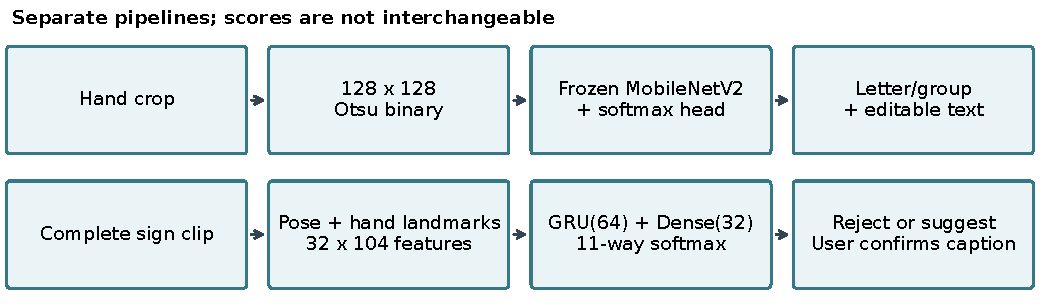
\includegraphics[width=\textwidth]{figures/pipeline.pdf}
\caption{\small Inference architecture. Static classification and complete-clip sentence recognition use separate feature contracts and label spaces. The original CNN comparison is specified in the method text. Manual confirmation is an interface safeguard, not evidence of recognition accuracy.}\label{fig:pipeline}
\end{figure}

\section{Models and training setup}
The reconstructed CNN uses two valid $5\times5$ convolutions with 32 filters, a $5\times5$ max-pooling layer and dropout 0.25. Two valid $3\times3$ convolutions with 64 filters follow, then $2\times2$ max pooling and dropout 0.25. Flattened features feed a 512-unit ReLU dense layer, dropout 0.5 and a softmax classifier. All convolutional layers use ReLU. The historical experiment has 36 outputs and preserves the architecture recorded in \texttt{ishara.py} at the thesis tag.

Adam uses its default learning rate of 0.001. Sparse categorical cross-entropy is minimised for 12 full epochs with batches of 18. Historical augmentation retains the surviving script's shear 0.2, zoom 0.2 and horizontal flips. These settings preserve the code record; horizontal flips require linguistic review because reflection can change a sign. Every training batch is visited in each epoch.

The comparison repeats the binary input across three channels and scales it to $[-1,1]$ for ImageNet MobileNetV2. Its backbone is frozen. Global average pooling produces 1,280-dimensional features, followed by dropout 0.2 and a new softmax head. Frozen features are cached once on CPU. The head is trained for 12 epochs using Adam, batch size 18 and no geometric augmentation. The exported end-to-end model still accepts image tensors, not cached vectors.

Pretraining and augmentation differ, so this is a transfer baseline rather than an architecture-only ablation. Both historical models share the exact split. The public run fits a separate head in its grouped label space.

Dependencies are pinned; TensorFlow seeds and deterministic operations are enabled on CPU. Reports record environment versions and model hashes. Floating-point results may still differ across processors and library versions.

\begin{figure}[!ht]\centering
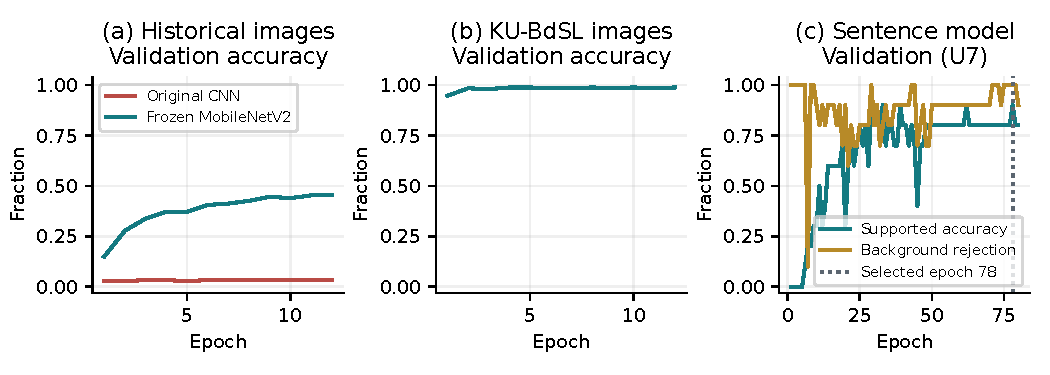
\includegraphics[width=\textwidth]{figures/validation-curves.pdf}
\caption{\small Unsmoothed validation histories from the saved runs. Panels (a) and (b) show all 12 image-training epochs. Panel (c) shows all 80 temporal epochs and the checkpoint selected using U7 validation. Test clips are not plotted or used for checkpoint selection. Training accuracy is omitted because the historical logger records the last batch rather than an epoch aggregate.}\label{fig:curves}
\end{figure}

\section{Metrics}
Test predictions are obtained once by argmax of each output distribution. Accuracy is the number correct divided by test support. Per-class precision, recall and F1 are reported with support; undefined values are set to zero. The confusion matrices contain raw counts and use the saved class order. Softmax outputs are presented as uncalibrated scores, never as a validated probability of correctness.

\section{Static classification results}
\begin{table}[!ht]\centering
\caption{Static classification on fixed image-level test partitions. Historical models share one split; KU-BdSL is a separate task.}\label{tab:static}
\resizebox{\textwidth}{!}{\begin{tabular}{lrrrrrr}\toprule Experiment & Classes & Train & Val. & Test & Acc. (\%) & Macro F1 \\\midrule
original & 36 & 709 & 148 & 148 & 3.38 & 0.0018 \\
mobilenet & 36 & 709 & 148 & 148 & 52.70 & 0.5072 \\
ku-mobilenet & 30 & 1020 & 240 & 240 & 99.58 & 0.9958 \\
\bottomrule\end{tabular}}
\end{table}
The historical comparison measures two models on the same image-level split. The public-data row uses a different collection and grouped label space and should be interpreted separately. These are additional experimental measurements, reported independently of the original preprint's accuracy statements. One seed and one run per configuration do not establish robustness or a confidence interval over training variability.

\begin{figure}[!ht]\centering
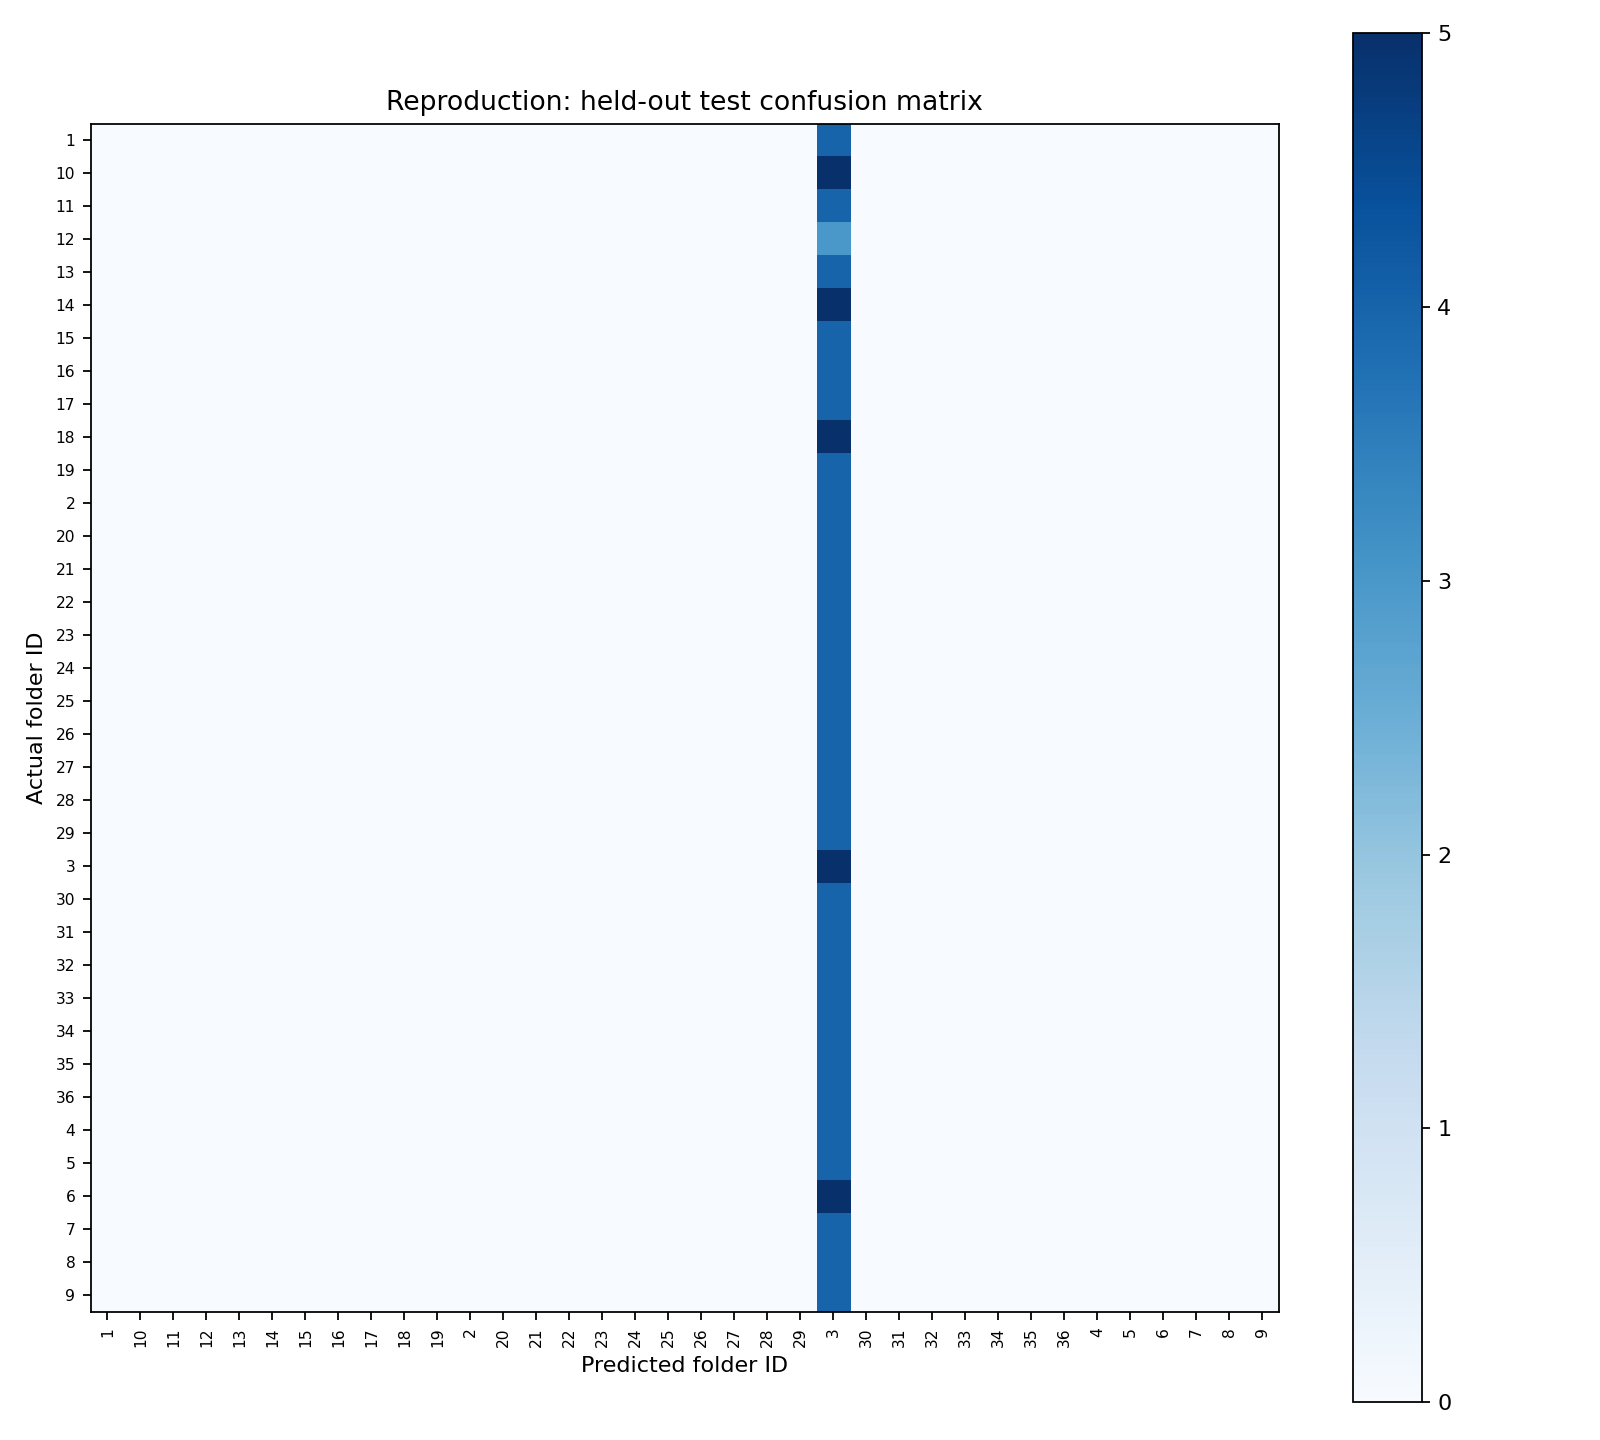
\includegraphics[width=.78\textwidth]{figures/original-confusion.png}
\caption{Historical CNN confusion matrix for 148 test images. Rows denote actual folder IDs and columns denote predicted IDs; entries are raw counts.}\label{fig:historical-confusion}
\end{figure}
Figure~\ref{fig:historical-confusion} shows held-out predictions; the raw counts are available as CSV. Concentration in a small number of prediction columns indicates poor discrimination across the historical classes.

Differences in image quality, class definitions and collection conditions prevent attributing cross-dataset score differences to model quality alone.

\section{Per-class metrics}
The following are the complete per-class precision (P), recall (R), F1 and support (N), rounded only for display. Unrounded values are in the committed CSV and JSON reports. The numeric IDs preserve the original folder labels; hyphenated public IDs denote grouped characters. Class order in the model and plots is lexicographic and stored explicitly.

\begin{minipage}[t]{.46\textwidth}\centering\renewcommand{\arraystretch}{.90}\textbf{Historical CNN}\\[5pt]\footnotesize\begin{tabular}{lrrrr}\toprule ID & P & R & F1 & N \\\midrule
1 & 0.000 & 0.000 & 0.000 & 4 \\
10 & 0.000 & 0.000 & 0.000 & 5 \\
11 & 0.000 & 0.000 & 0.000 & 4 \\
12 & 0.000 & 0.000 & 0.000 & 3 \\
13 & 0.000 & 0.000 & 0.000 & 4 \\
14 & 0.000 & 0.000 & 0.000 & 5 \\
15 & 0.000 & 0.000 & 0.000 & 4 \\
16 & 0.000 & 0.000 & 0.000 & 4 \\
17 & 0.000 & 0.000 & 0.000 & 4 \\
18 & 0.000 & 0.000 & 0.000 & 5 \\
19 & 0.000 & 0.000 & 0.000 & 4 \\
2 & 0.000 & 0.000 & 0.000 & 4 \\
20 & 0.000 & 0.000 & 0.000 & 4 \\
21 & 0.000 & 0.000 & 0.000 & 4 \\
22 & 0.000 & 0.000 & 0.000 & 4 \\
23 & 0.000 & 0.000 & 0.000 & 4 \\
24 & 0.000 & 0.000 & 0.000 & 4 \\
25 & 0.000 & 0.000 & 0.000 & 4 \\
26 & 0.000 & 0.000 & 0.000 & 4 \\
27 & 0.000 & 0.000 & 0.000 & 4 \\
28 & 0.000 & 0.000 & 0.000 & 4 \\
29 & 0.000 & 0.000 & 0.000 & 4 \\
3 & 0.034 & 1.000 & 0.065 & 5 \\
30 & 0.000 & 0.000 & 0.000 & 4 \\
31 & 0.000 & 0.000 & 0.000 & 4 \\
32 & 0.000 & 0.000 & 0.000 & 4 \\
33 & 0.000 & 0.000 & 0.000 & 4 \\
34 & 0.000 & 0.000 & 0.000 & 4 \\
35 & 0.000 & 0.000 & 0.000 & 4 \\
36 & 0.000 & 0.000 & 0.000 & 4 \\
4 & 0.000 & 0.000 & 0.000 & 4 \\
5 & 0.000 & 0.000 & 0.000 & 4 \\
6 & 0.000 & 0.000 & 0.000 & 5 \\
7 & 0.000 & 0.000 & 0.000 & 4 \\
8 & 0.000 & 0.000 & 0.000 & 4 \\
9 & 0.000 & 0.000 & 0.000 & 4 \\
\bottomrule\end{tabular}\end{minipage}\hfill
\begin{minipage}[t]{.51\textwidth}\centering\renewcommand{\arraystretch}{.90}\textbf{Public-data MobileNetV2}\\[5pt]\footnotesize\begin{tabular}{lrrrr}\toprule ID & P & R & F1 & N \\\midrule
2433 & 1.000 & 1.000 & 1.000 & 8 \\
2434 & 1.000 & 1.000 & 1.000 & 8 \\
2435 & 1.000 & 1.000 & 1.000 & 8 \\
2453 & 1.000 & 1.000 & 1.000 & 8 \\
2454 & 1.000 & 1.000 & 1.000 & 8 \\
2455 & 1.000 & 1.000 & 1.000 & 8 \\
2456 & 1.000 & 1.000 & 1.000 & 8 \\
2457 & 1.000 & 1.000 & 1.000 & 8 \\
2458 & 1.000 & 1.000 & 1.000 & 8 \\
2459 & 1.000 & 1.000 & 1.000 & 8 \\
2460-2479 & 1.000 & 1.000 & 1.000 & 8 \\
2461 & 1.000 & 1.000 & 1.000 & 8 \\
2462 & 1.000 & 0.875 & 0.933 & 8 \\
2463 & 1.000 & 1.000 & 1.000 & 8 \\
2464 & 1.000 & 1.000 & 1.000 & 8 \\
2465 & 1.000 & 1.000 & 1.000 & 8 \\
2466 & 1.000 & 1.000 & 1.000 & 8 \\
2467-2472 & 1.000 & 1.000 & 1.000 & 8 \\
2468-2510 & 1.000 & 1.000 & 1.000 & 8 \\
2469 & 1.000 & 1.000 & 1.000 & 8 \\
2470 & 1.000 & 1.000 & 1.000 & 8 \\
2471 & 1.000 & 1.000 & 1.000 & 8 \\
2474 & 1.000 & 1.000 & 1.000 & 8 \\
2475 & 1.000 & 1.000 & 1.000 & 8 \\
2476-2477 & 1.000 & 1.000 & 1.000 & 8 \\
2478 & 1.000 & 1.000 & 1.000 & 8 \\
2480-2524-2525 & 1.000 & 1.000 & 1.000 & 8 \\
2482 & 1.000 & 1.000 & 1.000 & 8 \\
2486-2488-2487 & 0.889 & 1.000 & 0.941 & 8 \\
2489 & 1.000 & 1.000 & 1.000 & 8 \\
\bottomrule\end{tabular}\end{minipage}

\vspace{10pt}The transfer comparison's complete 36-class table is distributed as \path{reports/mobilenet/per_class.csv}. The public matrix appears below; its axis labels are numeric Unicode/group IDs rather than inferred letter names.
\begin{figure}[!ht]\centering
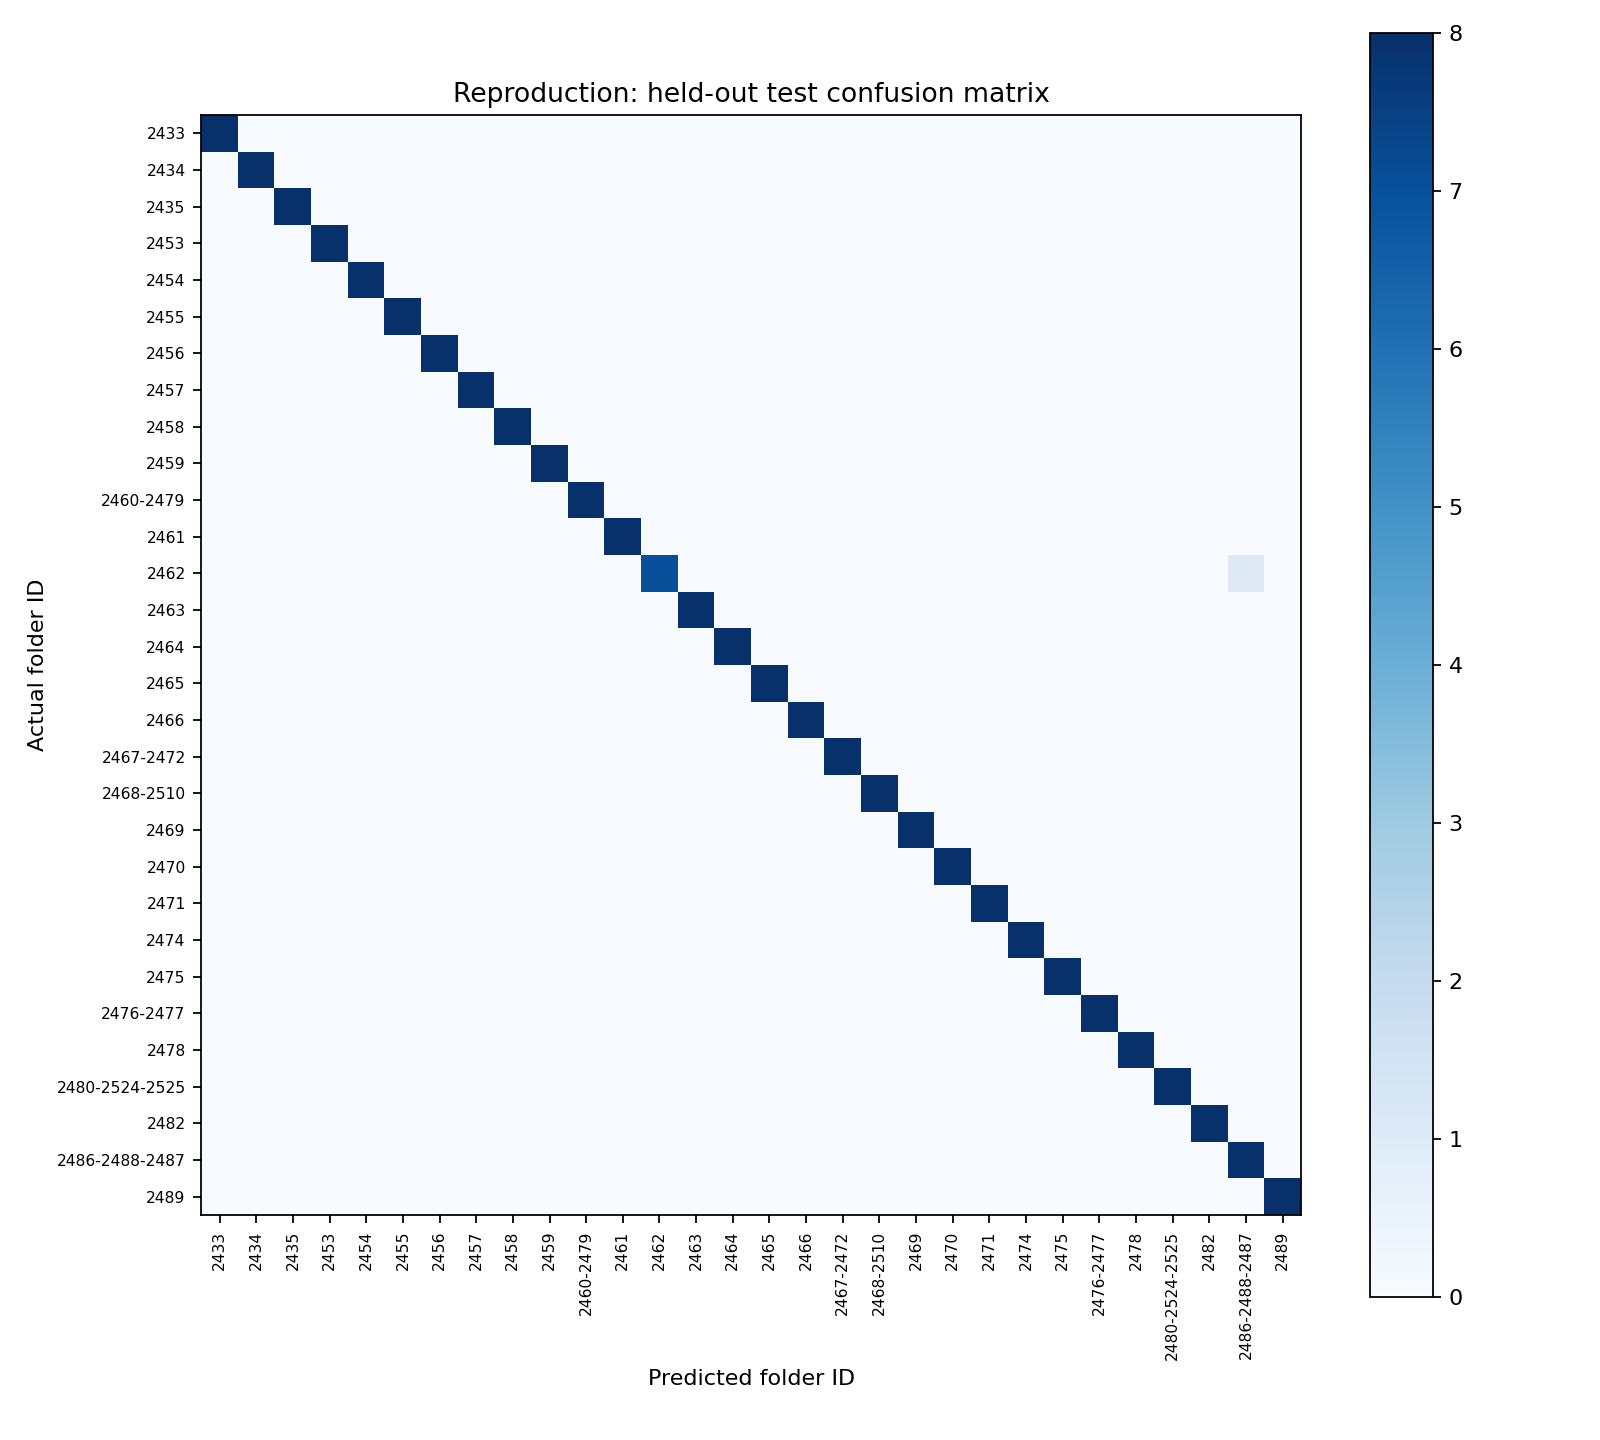
\includegraphics[width=.85\textwidth]{figures/ku-mobilenet-confusion.png}
\caption{KU-BdSL MobileNetV2 confusion matrix for 240 test images in 30 grouped classes. Rows are actual IDs and columns predicted IDs.}\label{fig:public-confusion}
\end{figure}

\section{Error analysis and qualitative evidence}
\begin{figure}[!ht]\centering
\begin{minipage}{.45\textwidth}\centering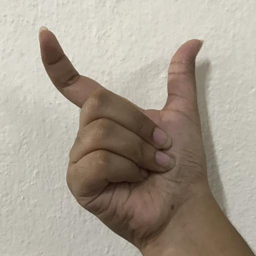
\includegraphics[height=3.2cm]{correct.png}\ Actual ID 2433; predicted 2433.\\ Score 100.0\%.\end{minipage}\hfill
\begin{minipage}{.45\textwidth}\centering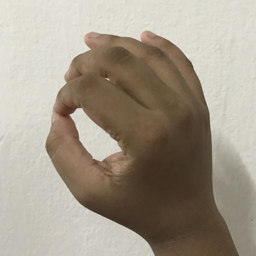
\includegraphics[height=3.2cm]{incorrect.png}\ Actual ID 2462; predicted 2486-2488-2487.\\ Score 25.5\%.\end{minipage}\hfill
\caption{A correct and an incorrect held-out KU-BdSL prediction. Scores are uncalibrated softmax outputs. Images: Jim et al., KU-BdSL v4, CC BY 4.0; resized derivatives.}\label{fig:examples}
\end{figure}

Figure~\ref{fig:examples} shows the first correct and first incorrect public test predictions in the saved manifest. These selected illustrations do not estimate error frequency. Source paths and unrounded scores are supplied in \texttt{examples.json}; the results page exposes every test prediction, including failures.

Competing handshapes, threshold sensitivity and cropping are plausible error sources, not established causes. Binary preprocessing removes colour and texture and may poorly match ImageNet features. An RGB baseline and controlled cropping ablation are future experiments, not measured improvements.
\section{Implementation and software validation}
The Python implementation provides command-line and PyQt5 interfaces for images, recorded video and cameras. Automated tests cover Otsu preprocessing, tensor contracts, image decoding, Keras prediction and video inference. Synthetic image and video fixtures test software behaviour independently of sign-recognition accuracy. Recorded-file sampling follows media timestamps, and tracking state resets between inputs.

The desktop video-input flow was also tested with a supported clip, a background false accept and a cropped BRAC tutorial greeting. The supported clip was recognised correctly; both unsupported inputs produced incorrect supported captions, including a coffee-related sentence for the greeting. Suggestions required confirmation before transcript insertion. No weights or thresholds were adjusted after these checks. The first two clips were previously evaluated examples, so this test measures integration consistency rather than new recognition accuracy. A separate letter-composition demonstration uses selected correctly classified held-out images; it is not continuous signing.

\section{Moving-phrase feasibility experiment}
A CPU prototype uses shoulder-normalised upper-body and hand landmarks from cropped Grameenphone and BRAC tutorial segments, with MediaPipe~\cite{hands} tracking and dynamic time warping. Ten phrases have one reference clip each from the first tutorial. A different signer in the second tutorial supplies four supported and eight unsupported segments. Printed captions inform manual annotations but are excluded from model features.

A distance threshold of 0.20 and relative margin of 0.10, specified before evaluation, yield 1/4 supported phrases recognised and 4/8 unsupported segments rejected. These small, manually segmented results demonstrate poor cross-signer discrimination, not validated continuous transcription. More signers, independent validation, representative unknown gestures and linguistic review are required. Complete segment annotations and errors accompany the code.

\subsection{Bounded sentence model}
A follow-up experiment uses 100 selected clips from the public Ban-Sign-Sent-9K-V1 repository (\url{https://huggingface.co/datasets/banglagov/Ban-Sign-Sent-9K-V1}). Ten text-diverse target sentences and ten background sentence types were selected before recognition outcomes. Encoded signer IDs U4/U5/U6 supply 60 training clips; U7 supplies 20 validation clips; U19 supplies 20 test clips. There is one clip per sentence and ID. Identity and consent were not independently verified, and the inspected dataset card has no explicit licence; source footage is not redistributed.

An 11-class GRU classifier (64 units, dropout 0.3, dense 32, softmax including background) uses 32-step motion/shape landmark sequences, Adam 0.001, batch 8, 80 epochs, temporal warp/noise augmentation and seed 2026. Validation selects the checkpoint and rejection threshold, with DTW as an alternative backend. The selected GRU obtains 6/10 supported captions correct and rejects 8/10 background clips on U19; 6 of 10 accepted captions are correct. The two false accepts illustrate the danger of confident captions. Background sentence types occur in training, so rejection does not establish novel-utterance detection. An earlier conservative baseline rejected all clips; its U19 outcome was already observed before this follow-up, which is exploratory rather than a wholly blind confirmation. Full clip-level predictions, class metrics and confusion counts accompany the code. Automatic sentence boundaries and general conversation translation remain unevaluated.

\begin{figure}[!ht]\centering
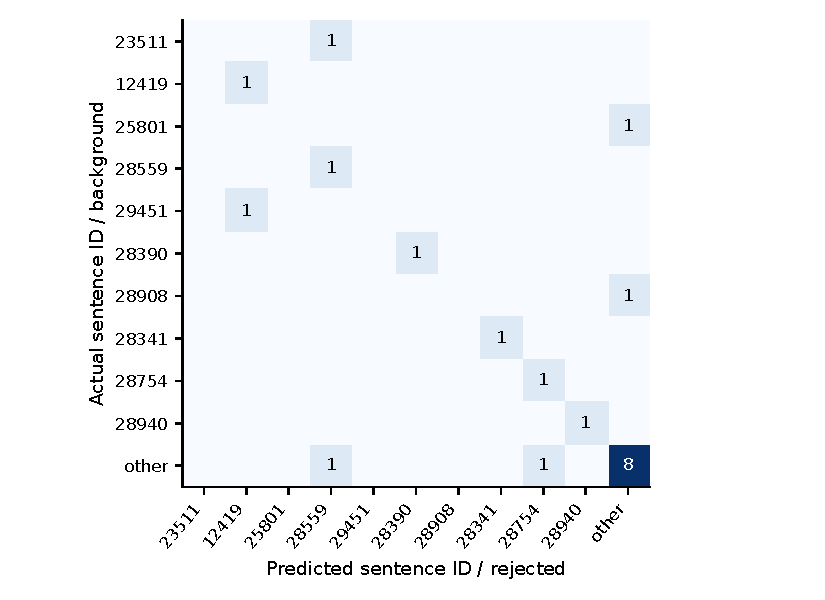
\includegraphics[width=.85\textwidth]{figures/sentence-confusion.pdf}
\caption{\small Raw confusion counts for 20 U19 sentence-test clips: one per supported sentence and ten background clips. Numeric IDs correspond to the published vocabulary manifest; ``other'' pools unsupported sentence types and rejected outputs. Six supported captions are correct, and eight background clips are rejected; two background clips are falsely captioned. Background types also occur in training, and a prior baseline outcome on this signer was observed.}\label{fig:sentence-confusion}
\end{figure}

\section{Limitations, ethics and accessibility}
Deployment evaluation requires Deaf-user-led task design, resolved data permissions and consent, independent signers and sessions, novel unsupported utterances, continuous-signing error analysis and measured end-to-end latency. These remain open research and validation requirements.

Small test supports make class metrics unstable. Neither static-image dataset permits a verified signer-disjoint partition in the layout used here, and capture-condition dependence can inflate image-level results. Historical annotations and their display mapping require expert review. The static classifier has no explicit unknown-sign, no-hand or out-of-distribution rejection class; the separate temporal background class does not solve arbitrary unknown recognition. A high softmax score can still be wrong.

KU-BdSL version 4 provides a documented CC BY 4.0 licence and participant-consent statement. That documentation does not transfer to the historical thesis images, whose consent records are absent. The software's MIT licence does not relicense third-party datasets. No unlicensed face video is incorporated. Historical paper text and figures remain under their original licence, and unchanged v1 is supplied for comparison.

Evaluation with Bangla Sign Language users must address signing practice, mobility, lighting, skin tone and camera access, following interdisciplinary guidance~\cite{bragg}. No such user study has been conducted; this system is not an evaluated replacement for interpreters.
\section{Code and data availability}
Code, pinned requirements, manifests, predictions and tests are available at \url{https://github.com/iamnajib71/Real-Time-Bangla-Sign-Language-Detector}. Versioned models, matching label maps and checksums are provided with release \texttt{v2.0.1}: \url{https://github.com/iamnajib71/Real-Time-Bangla-Sign-Language-Detector/releases/tag/v2.0.1}. KU-BdSL v4 is retrieved from its publisher~\cite{kudata} under CC BY 4.0 with SHA256 verification. Historical records and split manifests are preserved, but original consent documentation is unavailable. Ban-Sign-Sent source clips remain with the original provider; their reuse permissions are unresolved, and those clips are not redistributed.
\section{Changes from version 1}
The unchanged original preprint remains available. This version specifies the executable CNN, adds audited splits and prediction-level results, and reports separate public-data and temporal experiments. Earlier accuracy statements are not reused as measurements. Sparse-autoencoder, depth and MATLAB procedures lack executable evidence and are not reproduced.
\begin{thebibliography}{99}\small\setlength{\itemsep}{2pt}\setlength{\parskip}{0pt}
\bibitem{bragg} D. Bragg et al. Sign Language Recognition, Generation, and Translation: An Interdisciplinary Perspective. ASSETS, 16--31, 2019. DOI: \href{https://doi.org/10.1145/3308561.3353774}{10.1145/3308561.3353774}.
\bibitem{hassan} N. Hassan. Bangla Sign Language Gesture Recognition System: Using CNN Model. ScienceOpen Preprints, 2022. Non-peer-reviewed. DOI: \href{https://doi.org/10.14293/S2199-1006.1.SOR-.PPUF56Q.v1}{10.14293/S2199-1006.1.SOR-.PPUF56Q.v1}.
\bibitem{nsl2018} N. C. Camgoz, S. Hadfield, O. Koller, H. Ney and R. Bowden. Neural Sign Language Translation. CVPR, 7784--7793, 2018. DOI: \href{https://doi.org/10.1109/CVPR.2018.00812}{10.1109/CVPR.2018.00812}.
\bibitem{slt2020} N. C. Camgoz, O. Koller, S. Hadfield and R. Bowden. Sign Language Transformers: Joint End-to-End Sign Language Recognition and Translation. CVPR, 10020--10030, 2020. DOI: \href{https://doi.org/10.1109/CVPR42600.2020.01004}{10.1109/CVPR42600.2020.01004}.
\bibitem{survey} S. Alyami, H. Luqman and M. Hammoudeh. Reviewing 25 years of continuous sign language recognition research: Advances, challenges, and prospects. Information Processing \& Management 61(5), 103774, 2024. DOI: \href{https://doi.org/10.1016/j.ipm.2024.103774}{10.1016/j.ipm.2024.103774}.
\bibitem{kubdsl} A. A. J. Jim, I. Rafi, M. Z. Akon, U. Biswas and A.-A. Nahid. KU-BdSL: An open dataset for Bengali sign language recognition. Data in Brief 51, 109797, 2023. DOI: \href{https://doi.org/10.1016/j.dib.2023.109797}{10.1016/j.dib.2023.109797}.
\bibitem{kudata} A. A. J. Jim et al. KU-BdSL: Khulna University Bengali Sign Language dataset. Mendeley Data, version 4, 2023. DOI: \href{https://doi.org/10.17632/scpvm2nbkm.4}{10.17632/scpvm2nbkm.4}.
\bibitem{lipi} M. Hadiuzzaman, M. S. Ali, T. Sultana, A. R. Shafi, A. S. M. Miah and J. Shin. BAUST Lipi: A BdSL Dataset with Deep Learning Based Bangla Sign Language Recognition. arXiv preprint, 2024. DOI: \href{https://doi.org/10.48550/arXiv.2408.10518}{10.48550/arXiv.2408.10518}.
\bibitem{bdslw401} H. A. Rubaiyeat, N. Youssouf, M. K. Hasan and H. Mahmud. BdSLW401: Transformer-Based Word-Level Bangla Sign Language Recognition Using Relative Quantization Encoding (RQE). arXiv preprint, 2025. DOI: \href{https://doi.org/10.48550/arXiv.2503.02360}{10.48550/arXiv.2503.02360}.
\bibitem{dhrubo} T. H. Dhrubo, M. T. Reza, S. Sahariar and W. A. Mukto. Transformer based sign-to-text translation for Bangladeshi sign language. Scientific Reports 16, 1154, 2026. DOI: \href{https://doi.org/10.1038/s41598-025-30856-y}{10.1038/s41598-025-30856-y}.
\bibitem{sentence2025} A. D. Aishi, A. Das and M. F. Kader. From Gesture to Sentence: A Sentence-Level Translation Framework for Bangla Sign Language. ICCIT, 4675--4680, 2025. DOI: \href{https://doi.org/10.1109/ICCIT68739.2025.11491213}{10.1109/ICCIT68739.2025.11491213}.
\bibitem{mobilenet} M. Sandler, A. Howard, M. Zhu, A. Zhmoginov and L.-C. Chen. MobileNetV2: Inverted Residuals and Linear Bottlenecks. 2018. DOI: \href{https://doi.org/10.48550/arXiv.1801.04381}{10.48550/arXiv.1801.04381}.
\bibitem{hands} F. Zhang et al. MediaPipe Hands: On-device Real-time Hand Tracking. arXiv preprint, 2020. DOI: \href{https://doi.org/10.48550/arXiv.2006.10214}{10.48550/arXiv.2006.10214}.
\bibitem{otsu} N. Otsu. A Threshold Selection Method from Gray-Level Histograms. IEEE Transactions on Systems, Man, and Cybernetics 9(1), 62--66, 1979. DOI: \href{https://doi.org/10.1109/TSMC.1979.4310076}{10.1109/TSMC.1979.4310076}.
\end{thebibliography}
\end{document}
